\chapter{Categorical Syllogisms}\label{ch:catsyllogisms}
\markright{Ch. \ref{ch:catsyllogisms}: Categorical Syllogisms}

\newglossaryentry{categorical syllogism}
{
name=categorical syllogism,
description={An argument with two premises composed of categorical statements.}
}

\newglossaryentry{Aristotelian syllogism}
{
name=Aristotelian syllogism,
description={An argument where each statement is in one of the moods A, E, I, or O, and which has exactly three terms, arranged so that any two pairs of statements will share one term.}
}

\newglossaryentry{major term}
{
name=major term,
description={The term that is used as the predicate of the conclusion of an Aristotelian syllogism.}
}

\newglossaryentry{minor term}
{
name=minor term,
description={The term that is used as the subject of the conclusion of an Aristotelian syllogism.}
}

\newglossaryentry{middle term}
{
name=middle term,
description={The one term in an Aristotelian syllogism that does not appear in the conclusion.}
}

\newglossaryentry{major premise}
{
name=major premise,
description={The one premise in an Aristotelian syllogism that names the major term.}
}

\newglossaryentry{minor premise}
{
name=minor premise,
description={The one premise in an Aristotelian syllogism that names the minor term.}
}

\newglossaryentry{standard form}
{
name=standard form,
description={An Aristotelian syllogism that has been put into logically structured English with the following criteria: (1) all of the individual statements are in standard form, (2) each instance of a term is in the same format and is used in the same sense, and (3) the major premise appears first, followed by the minor premise, and then the conclusion.}
}

\newglossaryentry{conditional validity}
{
name=conditional validity,
description={A kind if validity that Aristotelian syllogisms have if they are valid only given the assumption that the objects named by its terms actually exist.}
}

\newglossaryentry{unconditional validity}
{
name=unconditional validity,
description={A kind of validity that an Aristotelian syllogism has regardless of whether the objects named by its terms actually exist.}
}


\section{Standard Form, Mood, and Figure}\label{sec:form_mood_figure}

So far we have just been looking at very short arguments using categorical statements. The arguments just had one premise and a conclusion that was often logically equivalent to the premise. For most of the history of logic in the West, however, the focus has been on arguments that are a step more complicated called \textsc{\glspl{categorical syllogism}}. A categorical syllogism is a two-premise argument composed of categorical statements. Aristotle began the study of this kind of argument in his book the \cite{Aristotle:prior}. This work was refined over the centuries by many thinkers in the Pagan, Christian, Jewish, and Islamic traditions until it reached the form it is in today.

There are actually all kinds of two-premise arguments using categorical statements, but Aristotle only looked at arguments where each statement is in one of the moods A, E, I, or O. The arguments also had to have exactly three terms, arranged so that any two pairs of statements will share one term. Let's call a categorical syllogism that fits this more narrow description an \textsc{\gls{Aristotelian syllogism}} Here is a typical Aristotelian syllogism using only mood-A sentences:

\begin{kormanize}
\premise{All mammals are vertebrates.}
\premise{All dogs are mammals.}
\conclusion{All dogs are vertebrates. }
\end{kormanize}
\label{AAA_arg}


Notice how the statements in this argument overlap each other. Each statement shares a term with the other two. Premise 2 shares its subject term with the conclusion and its predicate with Premise 1. Thus there are only three terms spread across the three statements. Aristotle dubbed these the major, middle, and minor premises, but there was initially some confusion about how to define them. In the 6th century, the Christian philosopher John Philoponus, drawing on the work of his pagan teacher Ammonius, decided to arbitrarily designate the \textsc{\gls{major term}} as the predicate of the conclusion, the \textsc{\gls{minor term}} as the subject of the conclusion, and the \textsc{\gls{middle term}} as the one term of the Aristotelian syllogism that does not appear in the conclusion. So in the argument above, the major term is ``vertebrate,'' the middle term is ``mammal,'' and the minor term is ``dog.'' We will adopt this convention as well.
We can also define the \textsc{\gls{major premise}} as the one premise in an Aristotelian syllogism that names the major term, and the \textsc{\gls{minor premise}} as the one premise that names the minor term. So in the argument above, Premise 1 is the major premise and Premise 2 is the minor premise.


With these definitions in place, we can now define the \textsc{\gls{standard form}} in logically structured English. Recall that in section~\ref{sec:QQDVD}, we started standardizing our language into something we called ``logically structured English'' in order to remove ambiguity and to make its logical structure clear. The first step was to define the standard form for a categorical statement, which we did on page \pageref{def:standard form}. Now we do the same thing for an Aristotelian syllogism. We say that an Aristotelian syllogism is in standard form for logically structured English if and only if these criteria have been met: (1) all of the individual statements are in standard form, (2) each instance of a term is in the same format and is used in the same sense, (3) the major premise appears first, followed by the minor premise, and then the conclusion.

\newglossaryentry{syllogism mood}
{
name=syllogism mood,
description={The classification of an Aristotelian syllogism based on the moods of statements it contains. The mood is designated simply by listing the three letters for the moods of the statements in the argument, such as AAA, EAE, AII, etc.}
}

Once we standardize things this way, we can actually catalog every possible form of an Aristotelian syllogism. To begin with, each of the three statements can take one of four forms: A, E, I, or O. This gives us $4 \times 4 \times 4,$ or 64 possibilities. These 64 possibilities are called the \textsc{\gls{syllogism mood}}, and we designate it just by writing the three letters of the moods of the statements that make it up. So the mood of the argument on page \pageref{AAA_arg} is simply AAA. All 64 moods are listed in table~\ref{tab:sixty_four_moods}, for reference.

\begin{table}[!ht]
\begin{tabu}{X[1,c] X[1,c] X[1,c] X[1,c]}
AAA & AAE & AAI & AAO \\
AEA & AEE & AEI & AEO \\
AIA & AIE & AII & AIO \\
AOA & AOE & AOI & AOO \\
EAA & EAE & EAI & EAO \\
EEA & EEE & EEI & EEO \\
EIA & EIE & EII & EIO \\
EOA & EOE & EOI & EOO \\
IAA & IAE & IAI & IAO \\
IEA & IEE & IEI & IEO \\
IIA & IIE & III & IIO \\
IOA & IOE & IOI & IOO \\
OAA & OAE & OAI & OAO \\
OEA & OEE & OEI & OEO \\
OIA & OIE & OII & OIO \\
OOA & OOE & OOI & OOO \\
\end{tabu}
\caption{The sixty-four moods of the Aristotelian syllogism}
\label{tab:sixty_four_moods}
\end{table}

In addition to varying the kind of statements we use in an Aristotelian syllogism, we can also vary the placement of the major, middle, and minor terms. There are four ways we can arrange them that fit the definition of an Aristotelian syllogism in standard form, shown in Table \ref{tab:four_figures}. Here $P$ stands for the major term, $S$ for the minor term, and $M$ for the middle. The thing to pay attention to is the placement of the middle terms. In figure 1, the middle terms form a line slanting down to the right. In figure 2, the middle terms are both pushed over to the right. In figure 3, they are pushed to the left, and in figure 4, they slant in the opposite direction from figure 1.

\begin{table}[!ht]
\begin{tabu}{X[1,c] X[1,c]}
\begin{kormanize}
\premise{\textbf{M} \hspace{1em} $P$}
\premise{$S$ \hspace{1em} \textbf{M}}
\conclusion{\hspace{.3ex} $S$ \hspace{1em} $P$}
\end{kormanize}

&

\begin{kormanize}
\premise{$P$ \hspace{1em} \textbf{M}}
\premise{$S$ \hspace{1em} \textbf{M}}
\conclusion{ \hspace{.3ex} $S$ \hspace{1em} $P$}
\end{kormanize}

\\

\hspace{2em} Figure 1

&

\hspace{2em} Figure 2

\\

\begin{kormanize}
\premise{\textbf{M} \hspace{1em} $P$}
\premise{\textbf{M} \hspace{1em} $S$}
\conclusion{ \hspace{.3ex}$S$ \hspace{1em} $P$}
\end{kormanize}

&

\begin{kormanize}
\premise{$P$ \hspace{1em} \textbf{M}}
\premise{\textbf{M} \hspace{1em} $S$}
\conclusion{\hspace{.3ex} $S$ \hspace{1em} $P$}
\end{kormanize}

\\

\hspace{2em} Figure 3

&

\hspace{2em} Figure 4

\end{tabu}

\caption{The four figures of the Aristotelian syllogism}
\label{tab:four_figures}
\end{table}

The combination of 64 moods and 4 figures gives us a total of 256 possible Aristotelian syllogisms. We can name them by simply giving their mood and figure. So this is OAO-3:

\begin{kormanize}
\premise{Some $M$ are not $P$.}
\premise{All $M$ are $S$.}
\conclusion{Some $S$ are not $P$.}
\end{kormanize}

Syllogism OAO-3 is a valid argument. We will be able to prove this with Venn diagrams in the next section. For now just read it over and try to see intuitively why it is valid. Most of the 256 possible syllogisms, however, are not valid.  In fact, most of them, like IIE-2, are quite obviously invalid:

\begin{kormanize}
\premise{Some $P$ are $M.$}
\premise{Some $S$ are $M.$}
\conclusion{No $S$ are $P.$}
\end{kormanize}

Given an Aristotelian syllogism in ordinary English, we can transform it into standard form in logically structured English and identify its mood and figure. Consider the following:

\begin{quotation}
\noindent No geckos are cats. I know this because all geckos are lizards, but cats aren't lizards.
\end{quotation}

The first step is to identify the conclusion, using the basic skills you acquired back in Chapter \ref{ch:what_is_logic}. In this case, you can see that ``because'' is a premise indicator word, so the statement before it, ``No geckos are cats,'' must be the conclusion.

Step two is to identify the major, middle, and minor terms. Remember that the major term is the predicate of the conclusion, and the minor term is the subject. So here the major term is ``cats,'' the minor term is ``geckos.'' The leftover term, ``lizards,'' must then be the middle term.

We show that we have identified the major, middle, and minor terms by writing a \gls{translation key}\label{def:translation_key}. As we saw on page \pageref{def:translation_key} a translation key is just a list that assigns English phrases or sentences to variable names. For categorical syllogism, this means matching the English phrases for the terms with the variables $S$, $M$, and $P$.

\begin{description}
\item[$S$ (minor term):] Geckos
\item[$M$ (middle term):] Lizards
\item[$P$ (major term):] Cats
\end{description}

Step three is to write the argument in canonical form using variables for the terms. The last statement, ``cats aren't lizards,'' is the major premise, because it has the major term in it. We need to change it to standard form, however, before we substitute in the variables. So first we change it to ``No cats are lizards.'' Then we write ``No $S$ are $M$.'' For the minor premise and the conclusion we can just substitute in the variables, so we get this:

\begin{kormanize}
\premise{No $P$ are $M$.}
\premise{All $S$ are $M$.}
\conclusion{ No $S$ are $P$.}
\end{kormanize}

Step four is to identify mood and figure. We can see that this is figure 2, because the middle term is in the predicate of both premises. Looking at the form of the sentences tells us that this is EAE.

\section{Testing Validity}\label{sec:testing_validity}

We have seen that there are 256 possible categorical arguments that fit Aristotle's requirements. Most of them are not valid. In this section, we will learn to use Venn diagrams to sort the valid arguments from the invalid. The method we will use is simply an extension of what we did in the last chapter, except with three circles instead of two.

\subsection{Venn Diagrams for Single Propositions}

In the previous chapter, we drew Venn diagrams with two circles for arguments that had had two terms. The circles partially overlapped, giving us four areas, each of which represented a way an individual could relate to the two classes. So area 1 represented things that were $S$ but not $P$, etc.

\begin{figure}
\centering
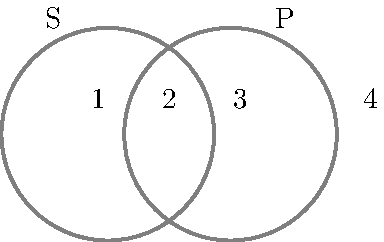
\includegraphics[width=0.6\textwidth]{2venn0}
\end{figure}

Now that we are considering arguments with three terms, we will need to draw three circles, and they need to overlap in a way that will let us represent the eight possible ways an individual can be inside or outside these three classes.

\begin{figure}
    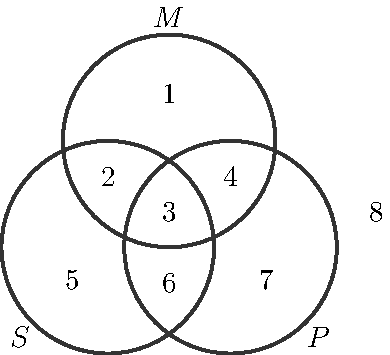
\includegraphics[width=0.6\textwidth]{3venn0}
\end{figure}

So in this diagram, area 1 represents the things that are $M$ but not $S$ or $P$, area 2 represents the things that are $M$ and $S$ but not $P$, etc. We'll mostly ignore region 8 as things that are neither $S$, nor $M$, nor $P$.

As before, we represent universal statements by filling in the area that the statement says cannot be occupied. The only difference is that now there are more possibilities. So, for instance, there are now four mood-A propositions that can occur in the two premises. The major premise can either be ``All $P$ are $M$'' or ``All $M$ are $P$,'' and the minor premise can be either ``All $S$ are $M$'' or ``All $M$ are $S$.'' The Venn diagrams for those four sentences are given in figure~\ref{fig:mood-A_venns}.

%\begin{figure*}
%\begin{tabu}{X[] X[1]}

%\caption{The four Venn diagrams for mood A sentences.}
%\label{fig:mood-A_venns}
%\end{tabu}
%\end{figure*}

Similarly, there are four mood-E propositions that can occur in the premises of an Aristotelian syllogism: ``No $P$ are $M$,'' ``No $M$ are $P$,'' ``No $S$ are $M$,'' and ``No $M$ are $S$.'' And again, we diagram these by shading out overlap between the two relevant circles. In this case, however, the first two statements are equivalent by conversion, as are the second two. Thus we only have two diagrams to worry about. See figure~\ref{fig:mood-E_venns}

%\begin{figure*}
%\begin{tabu}{X[1] X[1]}

%\caption{The two Venn diagrams for mood E sentences.}
%\label{fig:mood-E_venns}
%\end{tabu}
%\end{figure*}

Particular propositions are a bit trickier. Consider the statement ``Some $M$ are $P$.'' With a two circle diagram, you would just put an x in the overlap between the $M$ circle and the $P$ circle. But with the three circle diagram, there are now two places we can put it. It can go in either area 3 or area 4:

%\begin{figure}
%\centering

%\end{figure}

The solution here will be to put the x on the boundary between areas 3 and 4, to represent the fact that it could go in either location.

%\begin{figure}
%\centering

%\end{figure}

Sometimes, however, you won't have to draw the x on a border between two areas, because you will already know that one of those areas can't be occupied. Suppose, for instance, that you want to diagram ``Some $M$ are $P$,'' but you already know that all $M$ are $S$. You would diagram ``All $M$ are $S$'' like this:

%\begin{figure}
%\centering

%\end{figure}
Then, when it comes time to add the x for ``Some $M$ are $P$,'' you know that it has to go in the exact center of the diagram:

%\begin{figure}
%\centering

%\end{figure}

The Venn diagrams for the particular premises that can appear in Aristotelian syllogisms are given in figure~\ref{fig:part_venns}. The figure assumes that you are just representing the individual premises, and don't know any other premises that would shade some regions out. Again, some of these premises are equivalent by conversion, and thus share a Venn diagram.

%\begin{figure*}
%\centering
%\begin{tabu}{X[1] X[1]}

%\end{tabu}
%\caption{Basic Venn diagrams for all categorical sentences.}
%\label{fig:part_venns}
%\end{figure*}

\subsection{Venn Diagrams for Full Syllogisms}

In the last chapter, we used Venn diagrams to evaluate arguments with single premises. It turned out that when those arguments were valid, the conclusion was logically equivalent to the premise, so they had the exact same Venn diagram. This time we have two premises to diagram, and the conclusion won't be logically equivalent to either of them. Nevertheless we will find that for valid arguments, once we have diagrammed the two premises, we will also have diagrammed the conclusion.

First we need to specify a rule about the order to diagram the premises in: if one of the premises is universal and the other is particular, diagram the universal one first. This will allow us to narrow down the area where we need to put the x from the particular premise, as in the example above where we diagrammed ``Some $M$ are $P$'' assuming that we already knew that all $M$ are $S$.

Let's start with a simple example, an argument with the form AAA-1.

\begin{kormanize}
\premise{All $M$ are $P$.}
\premise{All $S$ are $M.$}
\conclusion{All $S$ are $P$.}
\end{kormanize}

Since both premises are universal, it doesn't matter what order we do them in. Let's do the major premise first. The major premise has us shade out the parts of the $M$ circle that don't overlap the $P$ circle, like this:

%\begin{figure}
%\centering

%\end{figure}

The second premise, on the other hand, tells us that there is nothing in the $S$ circle that isn't also in the $M$ circle. We put that together with the first diagram, and we get this:


%\begin{figure}
%\centering

%\end{figure}


From this we can see that the conclusion must be true. All $S$ are $P$, because the only space left in $S$ is the area in the exact center, area 7.

Now let's look at an argument that is invalid. One of the interesting things about the syllogism AAA-1 is that if you change the figure, it ceases to be valid. Consider AAA-2.

\begin{kormanize}
\premise{All $P$ are $M$.}
\premise{All $S$ are $M$.}
\conclusion{All $S$ are $P$.}
\end{kormanize}

Again, both premises are universal, so we can do them in any order, so we will do the major premise first. This time, the major premise tells us to shade out the part of $P$ that does not overlap $M$.


%\begin{figure}
%\centering

%\end{figure}


The second premise adds the idea that all $S$ are $M$, which we diagram like this:


%\begin{figure}
%\centering

%\end{figure}


Now we ask if the diagram of the two premises also shows that the conclusion is true. Here the conclusion is that all $S$ are $P$. If this diagram had made this true, we would have shaded out all the parts of $S$ that do not overlap $P$. But we haven't done that. It is still possible for something to be in area 5. Therefore this argument is invalid.

Now let's try an argument with a particular statement in the premises. Consider the argument IAI-1:

\begin{kormanize}
\premise{Some $M$ are $P$.}
\premise{All $S$ are $M$.}
\conclusion{Some $S$ are $P$.}
\end{kormanize}

Here, the second premise is universal, while the first is particular, so we begin by diagramming the universal premise.


%\begin{figure}
%\centering

%\end{figure}


Then we diagram the particular premise ``Some $M$ are $P$.'' This tells us that something is in the overlap between $M$ and $P$, but it doesn't tell us whether that thing is in the exact center of the diagram or in the area for things that are $M$ and $P$ but not $S$. Therefore, we place the x on the border between these two areas.


%\begin{figure}
%\centering

%\end{figure}


Now we can see that the argument is not valid. The conclusion asserts that something is in the overlap between $S$ and $P$. But the x we drew does not necessarily represent an object that exists in that overlap. There is something out there that could be in area 7, but it could just as easily be in area 6. The second premise doesn't help us, because it just rules out the existence of objects in areas 1 and 4.

For a final example, let's look at a case of a valid argument with a particular statement in the premises. If we simply change the figure of the argument in the last example from 1 to 3, we get a valid argument. This is the argument IAI-3:


\begin{kormanize}
\premise{Some $M$ are $P$.}
\premise{All $M$ are $S$.}
\conclusion{Some $S$ are $P$.}
\end{kormanize}

Again, we begin with the universal premise. This time it tells us to shade out part of the $M$ circle.


%\begin{figure}
%\centering

%\end{figure}



But now we fill in the parts of $M$ that don't overlap with $S$, we have to put the x in the exact center of the diagram.


%\begin{figure}
%\centering

%\end{figure}



And now this time we see that ``Some $S$ are $P$'' has to be true based on the premises, because the X has to be in area 3. So this argument is valid.

Using this method, we can show that 15 of the 256 possible syllogisms are valid. Remember, however, that the Venn diagram method uses \emph{Boolean assumptions about existential import}. If you make other assumptions about existential import, you will allow more valid syllogisms, as we will see in the next section. The additional syllogisms we will be able to prove valid in the next section will be said to have \textsc{\gls{conditional validity}} \label{def:Conditional_validity} because they are valid on the condition that the objects talked about in the universal statements actually exist. The 15 syllogisms that we can prove valid using the Venn diagram method have \textsc{\gls{unconditional validity}}. \label{def:Unconditional_validity} These syllogisms are given in Table \ref{tab:unconditionally_valid}.

\begin{table}
\begin{tabu}{X[1,c] X[1,c] X[1,c] X[1,c]}
\textbf{Figure 1} & \textbf{Figure 2} & \textbf{Figure 3} & \textbf{Figure 4} \\
Barbara (AAA)  & Camestres (AEE) & Disamis (IAI) & Calemes (AEE) \\
Celarent (EAE) & Cesare (EAE)    & Bocardo (OAO) & Dimatis (IAI) \\
Ferio (EIO)	   & Festino (EIO)   & Ferison (EIO) & Fresison (EIO) \\
Darii (AII)	   & Baroco (AOO)    & Datisi (AII)  & \\
\end{tabu}
\caption{The 15 unconditionally valid syllogisms.}
\label{tab:unconditionally_valid}
\end{table}
% the version of the naming scheme used here is just the one from wikipedia. Hurley gives a version of the poem, but doesn't say which one it is. He also doesn't use the names as he goes along. Hurley's list differs from the wikipedia list on three names: Ferioque for Ferio, Camenes for Calemes, Dimaris for Dimatis.

The names on Table~\ref{tab:unconditionally_valid} come from the Christian part of the Aristotelian tradition, where thinkers were writing in Latin. Students in that part of the tradition learned the valid forms by giving each one a name. The vowels in the name represented the mood of the syllogism. So B\textbf{a}rb\textbf{a}r\textbf{a} has the mood AAA, Fr\textbf{e}s\textbf{i}s\textbf{o}n has the mood EIO, etc. The consonants in each name were also significant: they related to a process the Aristotelians were interested in called reduction, where arguments in the later figures were shown to be equivalent to arguments in the first figure, which was taken to be more self-evident. We won't worry about reduction in this textbook, however. The names of the valid syllogisms were often worked into a mnemonic poem.

The oldest known version of the poem appears in a late 13th century book called \textit{Introduction to Logic} by William of Sherwood. Figure \ref{fig:barbara} is an image of the oldest surviving manuscript of the poem, digitized by the Bibliothèque Nationale de France.

The columns in Table \ref{tab:unconditionally_valid} represent the four figures. Syllogisms with the same mood also appear in the same row. So the EIO sisters---Ferio, Festino, Ferison, and Fresison---fill up row 3.  Camestres and Calemes share row 1;  Celarent and Cesare share row 2; and Darii and Datisi share row 4.

\begin{figure}[b]
\includegraphics*[scale=.75]{barbara}

\caption{The oldest surviving version of the ``Barbara, Celarent...'' poem, from William of Sherwood. The manuscript is held at the Biblioth\`eque Nationale de France, ms. Lat. 16617, \url{http://gallica.bnf.fr/ark:/12148/btv1b9066740r}}
\label{fig:barbara}
\end{figure}


\section*{Key Terms}
\begin{sortedlist}
\sortitem {Categorical syllogism}{}
\sortitem {Aristotelian syllogism}{}
\sortitem {Conditional validity}{}
\sortitem {Major premise}{}
\sortitem {Major term}{}
\sortitem {Middle term}{}
\sortitem {Minor premise}{}
\sortitem {Minor term}{}
\sortitem {Syllogism mood}{}
\sortitem {Standard form for an Aristotelian syllogism}{}
\sortitem {Translation key}{}
\sortitem {Unconditional validity}{}
\sortitem {Critical term}{}
\sortitem {Fallacy of exclusive premises}{}
\sortitem {Fallacy of illicit process}{}
\sortitem {Fallacy of particular premises}{}
\sortitem {Fallacy of the undistributed middle}{}
\sortitem {Negative-affirmative fallacy}{}

\end{sortedlist}
